\section{Analyse}
\subsection{Aufgabenstellung und direkte Anforderungen}
\label{aufgabenstellung}
Zu bearbeiten war Aufgabe Nr. 2, unter Verwendung von Methode Nr. 1, errechnet aus der Matrikelnummer.
Die Aufgabenstellung des Belegs besagt in diesem Fall, dass eine Materialverwaltung unter Verwendung der GTK-Bibliothek
für die Benutzeroberfläche programmiert werden soll.

\bigskip

\noindent
Aus der online verfügbaren, vollständigen Aufgabenstellung\footnote{\url{http://www.informatik.htw-dresden.de/~beck/PSPI/Belegaufgaben/},
abgerufen am 8.12.2016} können folgende direkte Anforderungen entnommen werden:

\begin{itemize}
\item Das Programm soll Datensätze verwalten -- also anlegen, sortiert tabellarisch auflisten, suchen, bearbeiten,
löschen sowie einzelne Datensätze anzeigen -- können
\item Ein Datensatz besteht hierbei aus Artikelbezeichnung, Artikelnummer und Lagerbestand
\item Die im Programm erfassten Daten sollen im Dateisystem gespeichert (bzw. davon wieder ausgelesen) werden können.
Hierbei ist nach klärendem Gespräch auch die Benutzung des Datenbanksystems SQLite erlaubt.
\item Der Lagerbestand soll explizit über einen gesonderten Menüpunkt veränderbar sein
\item Beim Verlassen der Anwendung sollen Daten, die sich während des Programmablaufs geändert werden
gespeichert werden können.\footnote{Eine kontinuierliche Speicherung ist hierbei nach klärendem Gespräch
zulässig}
\item Für die Umsetzung der Benutzeroberfläche muss zwingend die Bibliothek GTK+ verwendet werden
\item Es wird ein modularer Aufbau vorausgesetzt - Das Programm ist in mehrere sinnvolle, getrennt kompilierbare Module
zu unterteilen\footnote{Dies bedeutet m.E.n. eigene make-Targets für jedes Modul und schließt insbesondere nicht die
Nutzung gemeinsamer Typdefinitionen und Schnittstellen sowie gegenseitige Abhängigkeiten beim Linken der finalen
Anwendung aus}
Hierbei sind mindestens drei Module anzufertigen
\item Quelltexte sind sorgsam zu dokumentieren -- insbesondere ist die Urheberschaft im Programmkopf zu
kennzeichnen\footnote{Bei der Quellcodedokumentation richte ich mich nach \cite[Kap.4]{Martin:CleanCode}}
\item Das Programm muss auf den Laborrechnern der Fakultät Informatik an der HTW Dresden übersetz- und ausführbar sein.
\item Teil der Aufgabenstellung ist die verpflichtende Verwendung dynamischer Speicherverwaltung per malloc/free\footnote{
Ich werde den Einsatz von malloc/free dennoch auf das Notwendigste begrenzen, da gerade unter C die dynamische
Speicherverwaltung erfahrungsgemäß eine ergiebige Fehlerquelle darstellt.}
\end{itemize}

\subsection{Ergänzende Anforderungen}
Das oben genannte Minimum möchte ich außerdem noch um folgende Anforderungen ergänzen, die sich bei näherer Betrachtung
der Aufgabenstellung als sinnvoll und einfach umzusetzen bzw. allgemein als bewährte Verfahrensweise herausgestellt haben.

\begin{itemize}
\item Die Benutzeroberfläche soll selbsterklärend und fehlertolerant sein und möglichst wenig (also ideal überhaupt keine)
Nutzerdokumentation erfordern
\item Das Programm -- insbesondere die Module für Abstraktion, Speicherung und Verwaltung von Datensätzen (vgl.
Abschnitt \ref{datenabstraktionsschicht} ``\nameref{datenabstraktionsschicht}'', S. \pageref{datenabstraktionsschicht})
-- soll möglichst umfassend durch automatische Softwaretests abgedeckt werden.
Hierbei soll nach Möglichkeit auch das Vorgehen der Testgetriebenen Entwicklung (TDD) erprobt werden.
\item Dem Nutzer soll es ermöglicht werden, optional zu einem Datensatz auch ein Bild zu speichern
\item Die in GTK+ vorhandenen Schnittstellen zur Internationalisierung sollen genutzt werden.\footnote{Selbst wenn das
Programm praktisch gesehen wohl einsprachig bleiben wird, ist dies noch immer der für GTK+-Anwendungen übliche Weg
und mit vernachlässigbar wenig Mehraufwand umsetzbar.}
\item Das Speichern der Datenbankdatei soll auch unter neuem Dateinamen erfolgen können.
\item Der aktuell angezeigte Datensatz bzw. die aktuell angezeigte Auflistung sollen, wenn möglich, in ein CSV-basiertes
Format exportierbar sein.
\end{itemize}

\newpage
\subsection{Domänenmodell}
Ein einfaches, objektorientiertes Domänenmodell, welches obige Anforderungen unter Vernachlässigung dynamischer Aspekte
und Implementierungsdetails visualisiert, kann wie folgt aussehen:

\begin{center}
\noindent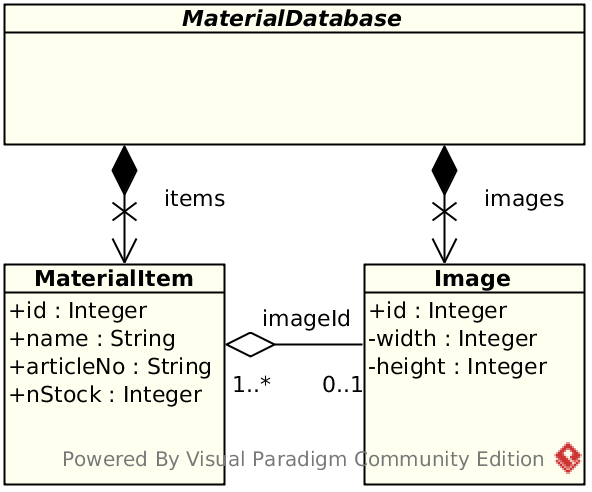
\includegraphics[width=110mm,keepaspectratio]{images/01-domaenenmodell.png}
\end{center}

Mögliche Erweiterungen dieses Modells für die Zukunft könnten beispielsweise die Katalogisierung der Materialdatensätze
in einem Kategoriebaum oder das Hinzufügen weitere Metadaten (u.A. auch Bilder) zu einem Datensatz sein.

\newpage
\subsection{Anwendungsfälle}
Die Kernanwendungsfälle, welche aus den Anforderungen entnommen werden können sind in folgendem Diagramm dargestellt:

\begin{center}
\noindent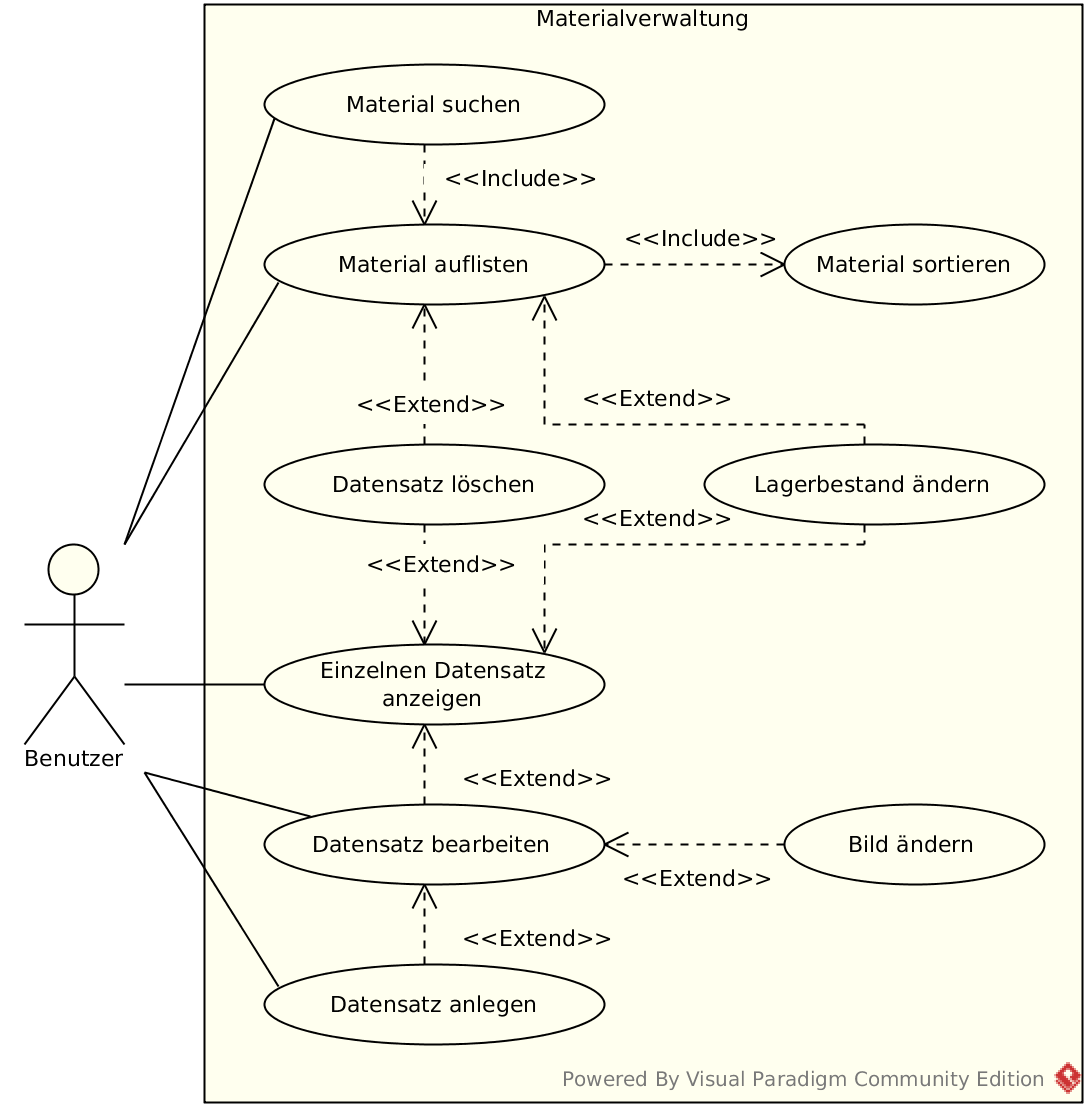
\includegraphics[width=150mm,keepaspectratio]{images/02-anwendungsfaelle.png}
\end{center}

Bereits hier zeigt sich eine möglicherweise sinnvolle Aufteilung in zwei Ansichten: Eine Such- und Katalogansicht,
sowie eine Detailansicht für einzelne Datensätze. Somit können sich beispielsweise Suche, Sortierung und Auflistung der
Materialdatensätze große Teile des Codes teilen und auch die Nutzeroberfläche bleibt in weiten Teilen kohärent und
für den Nutzer einleuchtend.

Eine Ausnahme stellt die Änderung des Lagerbestands dar: Dieser Anwendungsfall sollte von
beiden Ansichten aus erreichbar sein, denn der Lagerbestand wird im Vergleich zu allen anderen Teilen des Datensatzes
wohl mit Abstand am Häufigsten veränderbar sein und sollte daher mit möglichst wenig Aufwand auch aus der Übersichtsliste
erreichbar sein. Nichtsdestotrotz muss sich der Lagerbestand aber auch aus der Datensatz-Detailansicht heraus verändern
lassen können, soll diese doch eine vollständige Repräsentation und Manipulation eines einzelnen Datensatzes ermöglichen.

Doch auch das Löschen eines Datensatzes sollte aus beiden Ansichten heraus erreichbar sein. Zum Einen gehört es
zu einer vollständigen Datensatzmanipulation hinzu, dass ein Datensatz auch gelöscht werden kann, andererseits möchte
man als Nutzer einer Software nicht immer erst die Detailansicht eines Datensatzes aufrufen, um diesen (oder gar mehrere)
zu löschen.

Triviale Anwendungsfälle, welche keiner weiteren Erläuterung bedürfen, wurden in diesem Diagramm nicht berücksichtigt.